%
% volumen.tex
%
% (c) 2018 Prof Dr Andreas Müller, Hochschule Rapperswil
%
\documentclass[tikz]{standalone}
\usepackage{times}
\usepackage{amsmath}
\usepackage{txfonts}
\usepackage[utf8]{inputenc}
\usepackage{graphics}
\usepackage{color}
\usepackage{ifthen}
\usetikzlibrary{arrows,intersections,math}
\newboolean{showgrid}
\setboolean{showgrid}{true}
\begin{document}

\begin{tikzpicture}[>=latex,thick]

\node at (-3.8,0) {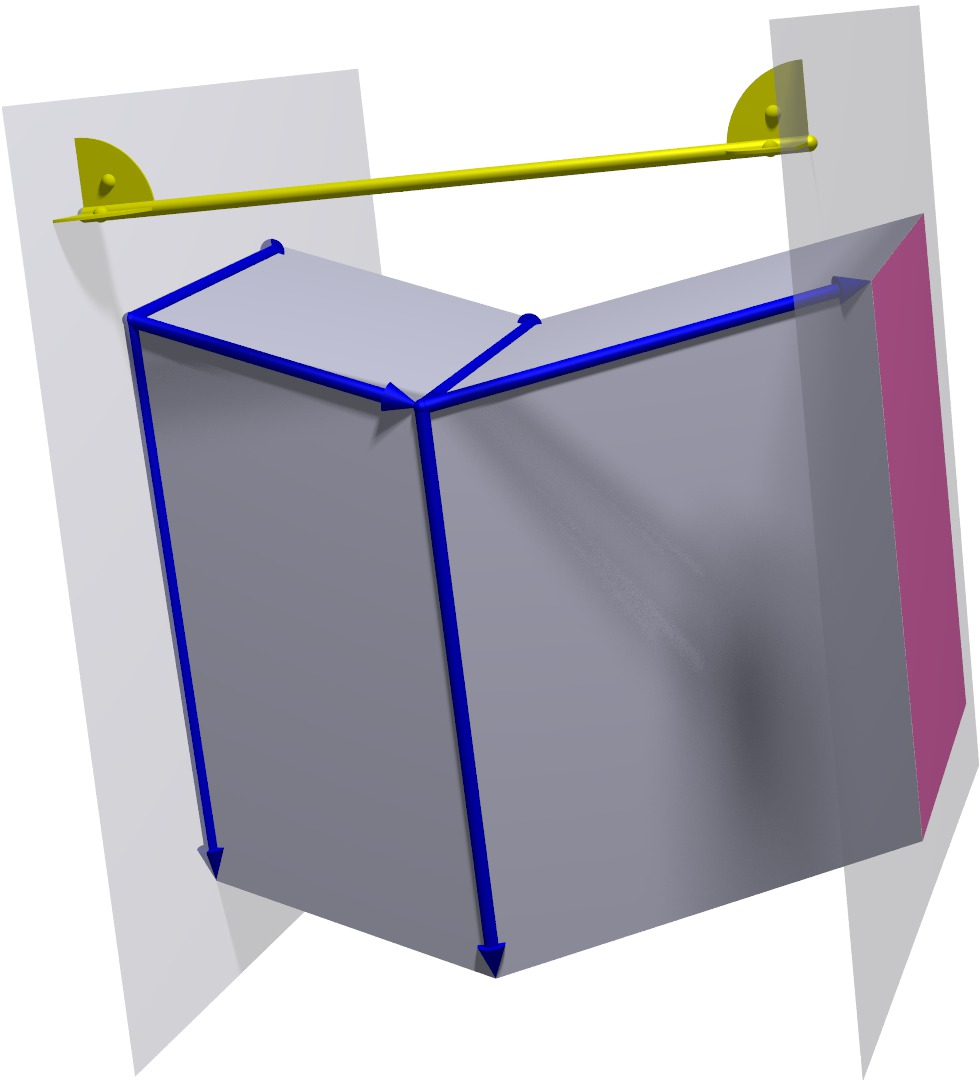
\includegraphics[width=6cm]{volumen1.jpg}};
\node at (+3.8,0) {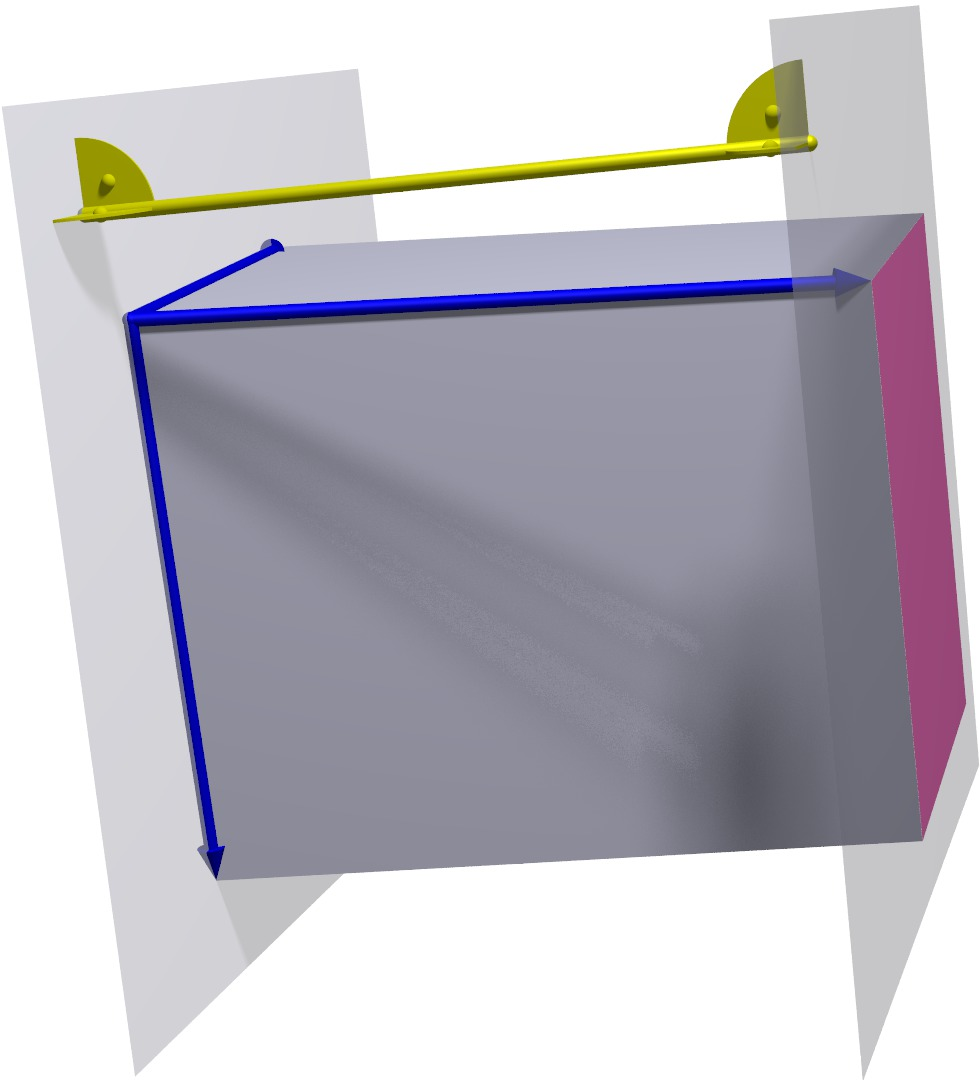
\includegraphics[width=6cm]{volumen2.jpg}};
\node at (0,0) {$=$};

% Gitter
\ifthenelse{\boolean{showgrid}}{
\draw[step=0.1,line width=0.1pt] (-7,-4) grid (7, 4);
\draw[step=0.5,line width=0.4pt] (-7,-4) grid (7, 4);
\draw (-7,-4) grid (7, 4);
\fill (0,0) circle[radius=0.05];
}{}

% Vektoren links
\node at (-6,-0.3) {$\vec{b}$};
\node at (-4.3,-0.9) {$\vec{b}$};

\node at (-5.4,1.9) {$\vec{c}$};
\node at (-3.8,1.4) {$\vec{c}$};

\node at (-5,1.3) {$\vec{a}'$};
\node at (-2.6,1.5) {$\vec{a}''$};

\node at (-4,2.5) {$h$};

% Vektoren rechts
\node at (2.2,1.9) {$\vec{c}$};
\node at (1.6,-0.3) {$\vec{b}$};
\node at (4,1.8) {$\vec{a}$};

\node at (3.6,2.5) {$h$};

\end{tikzpicture}

\end{document}
